\documentclass[11pt,compress,t,notes=noshow, xcolor=table]{beamer}
\usepackage[]{graphicx}\usepackage[]{color}
% maxwidth is the original width if it is less than linewidth
% otherwise use linewidth (to make sure the graphics do not exceed the margin)
\makeatletter
\def\maxwidth{ %
  \ifdim\Gin@nat@width>\linewidth
    \linewidth
  \else
    \Gin@nat@width
  \fi
}
\makeatother

\newcommand{\citebutton}[2]{%
\beamergotobutton{\href{#2}{#1}}%
}

\newcommand{\blu}[1]{\textcolor{blue}{#1}}
\newcommand{\org}[1]{\textcolor{orange}{#1}}
\newcommand{\ques}{\textbf{\textcolor{red}{Question:  }}}
\newcommand{\questionssofar}{\begin{frame}\frametitle{Any questions?}\end{frame}}

\newcommand\warning{%
 \makebox[1.4em][c]{%
 \makebox[0pt][c]{\raisebox{.1em}{\scriptsize!}}%
 \makebox[0pt][c]{\color{red}\normalsize$\bigtriangleup$}}}%

\definecolor{fgcolor}{rgb}{0.345, 0.345, 0.345}
\newcommand{\hlnum}[1]{\textcolor[rgb]{0.686,0.059,0.569}{#1}}%
\newcommand{\hlstr}[1]{\textcolor[rgb]{0.192,0.494,0.8}{#1}}%
\newcommand{\hlcom}[1]{\textcolor[rgb]{0.678,0.584,0.686}{\textit{#1}}}%
\newcommand{\hlopt}[1]{\textcolor[rgb]{0,0,0}{#1}}%
\newcommand{\hlstd}[1]{\textcolor[rgb]{0.345,0.345,0.345}{#1}}%
\newcommand{\hlkwa}[1]{\textcolor[rgb]{0.161,0.373,0.58}{\textbf{#1}}}%
\newcommand{\hlkwb}[1]{\textcolor[rgb]{0.69,0.353,0.396}{#1}}%
\newcommand{\hlkwc}[1]{\textcolor[rgb]{0.333,0.667,0.333}{#1}}%
\newcommand{\hlkwd}[1]{\textcolor[rgb]{0.737,0.353,0.396}{\textbf{#1}}}%
\let\hlipl\hlkwb

\usepackage{framed}
\makeatletter
\newenvironment{kframe}{%
 \def\at@end@of@kframe{}%
 \ifinner\ifhmode%
  \def\at@end@of@kframe{\end{minipage}}%
  \begin{minipage}{\columnwidth}%
 \fi\fi%
 \def\FrameCommand##1{\hskip\@totalleftmargin \hskip-\fboxsep
 \colorbox{shadecolor}{##1}\hskip-\fboxsep
     % There is no \\@totalrightmargin, so:
     \hskip-\linewidth \hskip-\@totalleftmargin \hskip\columnwidth}%
 \MakeFramed {\advance\hsize-\width
   \@totalleftmargin\z@ \linewidth\hsize
   \@setminipage}}%
 {\par\unskip\endMakeFramed%
 \at@end@of@kframe}
\makeatother

\definecolor{shadecolor}{rgb}{.97, .97, .97}
\definecolor{messagecolor}{rgb}{0, 0, 0}
\definecolor{warningcolor}{rgb}{1, 0, 1}
\definecolor{errorcolor}{rgb}{1, 0, 0}
\newenvironment{knitrout}{}{} % an empty environment to be redefined in TeX

\usepackage{alltt}
\newcommand{\SweaveOpts}[1]{}  % do not interfere with LaTeX
\newcommand{\SweaveInput}[1]{} % because they are not real TeX commands
\newcommand{\Sexpr}[1]{}       % will only be parsed by R
\newcommand{\xmark}{\ding{55}}%


\usepackage[english]{babel}
\usepackage[utf8]{inputenc}

\usepackage{dsfont}
\usepackage{verbatim}
\usepackage{amsmath}
\usepackage{amsfonts}
\usepackage{amssymb}
\usepackage{bm}
\usepackage{csquotes}
\usepackage{multirow}
\usepackage{longtable}
\usepackage{booktabs}
\usepackage{enumerate}
\usepackage[absolute,overlay]{textpos}
\usepackage{psfrag}
\usepackage{algorithm}
\usepackage{algpseudocode}
\usepackage{eqnarray}
\usepackage{arydshln}
\usepackage{tabularx}
\usepackage{placeins}
\usepackage{tikz}
\usepackage{setspace}
\usepackage{colortbl}
\usepackage{mathtools}
\usepackage{wrapfig}
\usepackage{bm}
\usepackage{amsmath}
\usepackage{pifont}

\usetikzlibrary{shapes.multipart,shapes,arrows,automata,positioning,calc,chains,trees, shadows}
\tikzset{
  %Define standard arrow tip
  >=stealth',
  %Define style for boxes
  punkt/.style={
    rectangle,
    rounded corners,
    draw=black, very thick,
    text width=6.5em,
    minimum height=2em,
    text centered},
  % Define arrow style
  pil/.style={
    ->,
    thick,
    shorten <=2pt,
    shorten >=2pt,}
}

\tikzstyle{vec}=[draw, rectangle, fill = white, minimum width=5mm, minimum height=1cm, inner sep = 2pt]

\usepackage{subfig}

% Defines macros and environments
\usepackage{../../style/lmu-lecture}


\let\code=\texttt
\let\proglang=\textsf

\setkeys{Gin}{width=0.9\textwidth}

\setbeamertemplate{frametitle}{\expandafter\uppercase\expandafter\insertframetitle}

\usepackage{bbm}
% basic latex stuff
\newcommand{\pkg}[1]{{\fontseries{b}\selectfont #1}} %fontstyle for R packages
\newcommand{\lz}{\vspace{0.5cm}} %vertical space
\newcommand{\dlz}{\vspace{1cm}} %double vertical space
\newcommand{\oneliner}[1] % Oneliner for important statements
{\begin{block}{}\begin{center}\begin{Large}#1\end{Large}\end{center}\end{block}}


%new environments
\newenvironment{vbframe}  %frame with breaks and verbatim
{
 \begin{frame}[containsverbatim,allowframebreaks]
}
{
\end{frame}
}

\newenvironment{vframe}  %frame with verbatim without breaks (to avoid numbering one slided frames)
{
 \begin{frame}[containsverbatim]
}
{
\end{frame}
}

\newenvironment{blocki}[1]   % itemize block
{
 \begin{block}{#1}\begin{itemize}
}
{
\end{itemize}\end{block}
}

\newenvironment{fragileframe}[2]{  %fragile frame with framebreaks
\begin{frame}[allowframebreaks, fragile, environment = fragileframe]
\frametitle{#1}
#2}
{\end{frame}}


\newcommand{\myframe}[2]{  %short for frame with framebreaks
\begin{frame}[allowframebreaks]
\frametitle{#1}
#2
\end{frame}}

\newcommand{\remark}[1]{
  \textbf{Remark:} #1
}


\newenvironment{deleteframe}
{
\begingroup
\usebackgroundtemplate{
\includegraphics[width=\paperwidth,height=\paperheight]{../style/color/red.png}}
 \begin{frame}
}
{
\end{frame}
\endgroup
}
\newenvironment{simplifyframe}
{
\begingroup
\usebackgroundtemplate{
\includegraphics[width=\paperwidth,height=\paperheight]{../style/color/yellow.png}}
 \begin{frame}
}
{
\end{frame}
\endgroup
}\newenvironment{draftframe}
{
\begingroup
\usebackgroundtemplate{
\includegraphics[width=\paperwidth,height=\paperheight]{../style/color/green.jpg}}
 \begin{frame}
}
{
\end{frame}
\endgroup
}
% https://tex.stackexchange.com/a/261480: textcolor that works in mathmode
\makeatletter
\renewcommand*{\@textcolor}[3]{%
  \protect\leavevmode
  \begingroup
    \color#1{#2}#3%
  \endgroup
}
\makeatother





\input{../../latex-math/basic-math.tex}
\input{../../latex-math/basic-ml.tex}

\newcommand{\titlefigure}{figure/bert.jpeg}
\newcommand{\learninggoals}{
\item Understand the use of the transformer encoder in this model
\item Understand the architectural components}

\title{BERT}
% \author{}
\institute{\href{https://slds-lmu.github.io/lecture_dl4nlp/}{slds-lmu.github.io/lecture\_dl4nlp}}
\date{}

\begin{document}
\lecturechapter{The Architecture}
\lecture{Deep Learning for NLP}

% ------------------------------------------------------------------------------

\begin{frame}{Predecessors of BERT}
\hbox{\hspace{-3em} 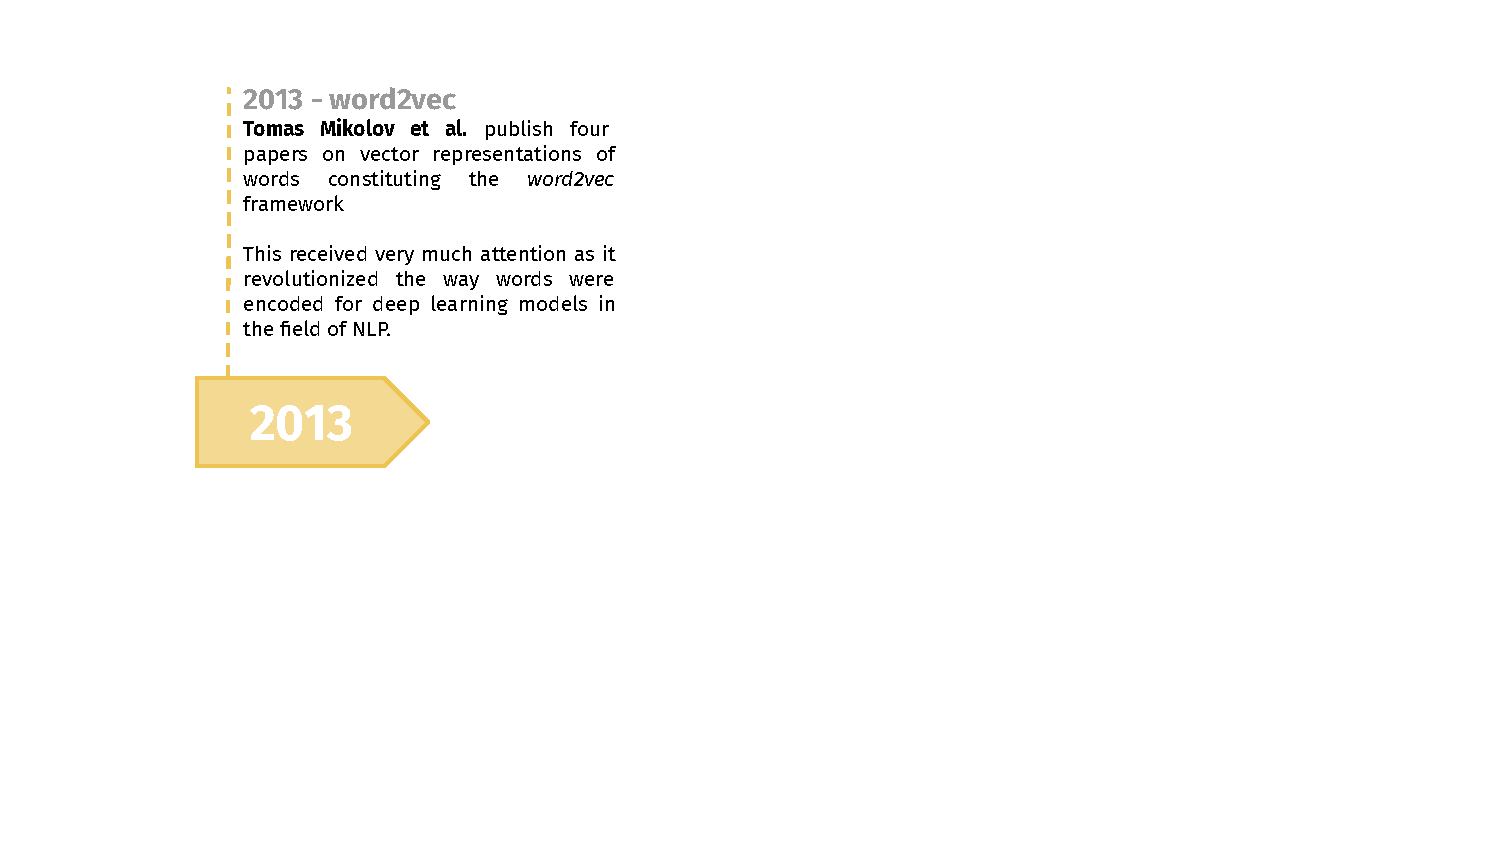
\includegraphics[width=12cm,page=1]{figure/transfer_learning_timeline1_nlp.pdf}}
\end{frame}
\begin{frame}[noframenumbering]{Predecessors of BERT}
\hbox{\hspace{-3em} \includegraphics[width=12cm,page=2]{figure/transfer_learning_timeline1_nlp.pdf}}
\end{frame}
\begin{frame}[noframenumbering]{Predecessors of BERT}
\hbox{\hspace{-3em} \includegraphics[width=12cm,page=3]{figure/transfer_learning_timeline1_nlp.pdf}}
\end{frame}
\begin{frame}[noframenumbering]{Predecessors of BERT}
\hbox{\hspace{-3em} \includegraphics[width=12cm,page=4]{figure/transfer_learning_timeline1_nlp.pdf}}
\end{frame}
\begin{frame}[noframenumbering]{Predecessors of BERT}
\hbox{\hspace{-3em} \includegraphics[width=12cm,page=5]{figure/transfer_learning_timeline1_nlp.pdf}}
\end{frame}

% ------------------------------------------------------------------------------

\begin{frame}{context: ulmfit and gpt}

\vfill

	\textbf{Shortcomings of ELMo:}

	\begin{itemize}
		\item No adaption of the Embeddings to target domain/task
		\item Sequential nature of LSTMs: Not fully parallelizable 
	\end{itemize}
	
	\textbf{Alleviations/Alternatives:}

	\begin{itemize}
		\item ULMFiT \citebutton{Howard and Ruder, 2018}{https://www.aclweb.org/anthology/P18-1031} is a uni-directional LSTM which is fine-tuned as a whole model on data from the target domain/task.
		\item GPT \citebutton{Radford et al., 2018}{https://s3-us-west-2.amazonaws.com/openai-assets/research-covers/language-unsupervised/language_understanding_paper.pdf} is a Transformer decoder which is fine-tuned as a whole model on data from the target domain/task.
	\end{itemize}
	
	\textbf{All three still not sufficient:}

	\begin{itemize}
		\item \textit{Bidirectionally contextual:} Only ELMo 
		\item \textit{Parallelizable:} Only GPT
		\item \textit{Fine-tune whole model:} Only ULMFiT \& GPT
	\end{itemize}
	
\vfill


\end{frame}

% ------------------------------------------------------------------------------

\begin{vbframe}{bert: key facts}

\vfill

\textit{\textbf{B}idirectional \textbf{E}ncoder \textbf{R}epresentations from \textbf{T}ransformers:}

\vspace{.5cm}

\begin{itemize}
		\item Bidirectionally contextual model\\
					$\to$ The embeddings of a single token depend on its left- and on its right-side context (similar to ELMo, but better)
		\item Completely replaces recurrent architectures by Self-Attention\\
					$\to$ parallelizable
		\item Model can fine-tuned as a whole
\end{itemize}

\vfill

\end{vbframe}

% ------------------------------------------------------------------------------

\begin{vbframe}{ELMo vs. GPT vs. BERT}

\vfill

\begin{figure}
\centering
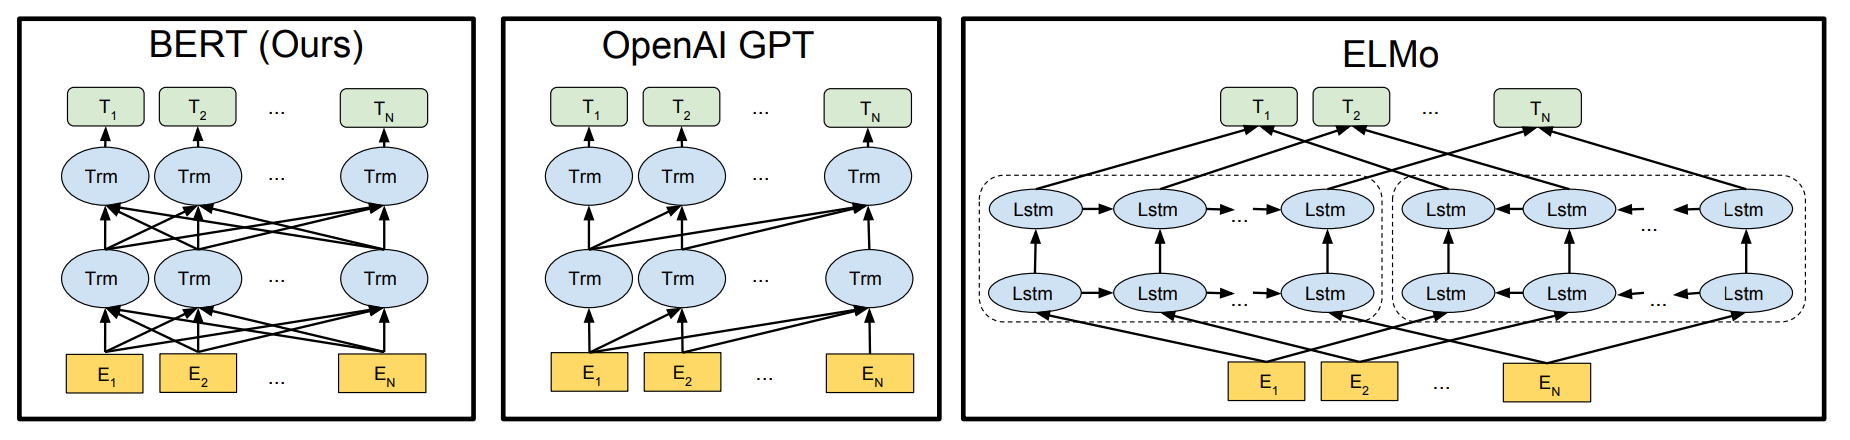
\includegraphics[width = 11cm]{figure/comparison-bert.png}\\ 
\citebutton{Source: Devlin et al., 2019}{https://aclanthology.org/N19-1423.pdf}
\end{figure}

\textbf{Major architectural differences:}

\begin{itemize}
\item ELMo uses two separate unidirectional models to achieve bidirectionality 
  $\rightarrow$ Only "\textit{shallow}" bidirectionality
\item GPT is not bidirectional, thus no issues concerning causality
\item BERT combines the best of both worlds: $$Self\text{-}Attention + (Deep)\;Bidirectionality$$
\end{itemize} 

\vfill

\end{vbframe}

% ------------------------------------------------------------------------------

\begin{vbframe}{bert: key facts}

\vfill

	\begin{itemize}
		\item New self-supervised objective(s)
		\item[] $\to$ MLM as \textit{necessity} for the architecture to work
		\item[] $\to$ Next-Sentence-Prediction as complementary objective\\(cf. next section)
		\item Transformer \textit{encoder} as backbone of the architecture
		\item 110M (340M) parameters in total for $BERT_{Base}$ ($BERT_{Large}$)
			\begin{itemize}
				\item 12 (24) Transformer encoder blocks
				\item Embedding size of $E = 768$ (1024)
				\item Hidden layer size $H = E$
				\item $A = H/64 = 12$ (16) attention heads
				\item Feed-forward size is set to $4H$
			\end{itemize}
	\end{itemize}

\vfill

\end{vbframe}

% ------------------------------------------------------------------------------

\begin{vbframe}{Core of BERT -- Transformer Encoder}

\begin{figure}
	\centering
		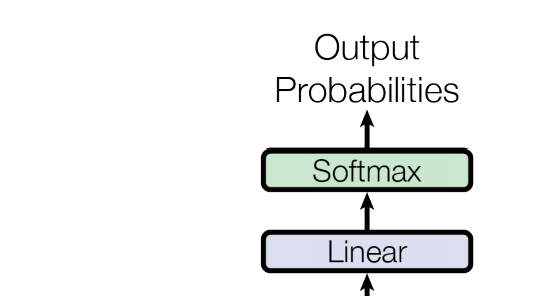
\includegraphics[width = 3cm]{figure/bert-top.png}\\ 
		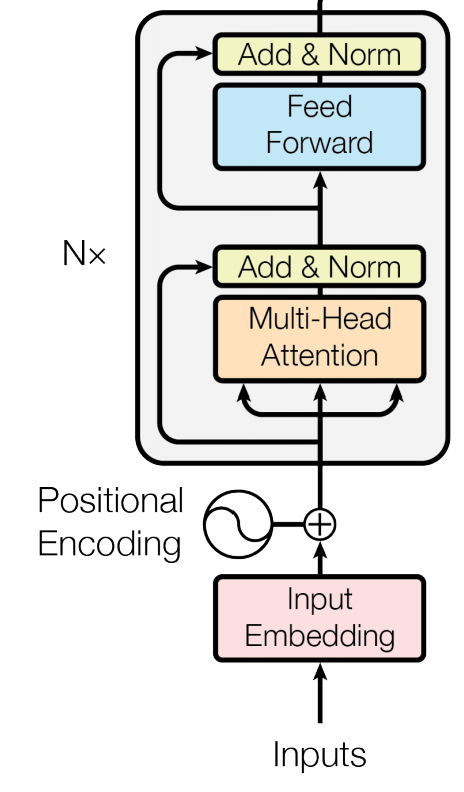
\includegraphics[width = 2.8cm]{figure/bert-bottom.png}\\ 
	\citebutton{Vaswani et al. (2017)}{https://arxiv.org/pdf/1706.03762.pdf}
\end{figure}

\end{vbframe}

% ------------------------------------------------------------------------------

\begin{frame}{A remark on "Causality"}

\vfill

\textbf{Causality is an issue!}
	
\begin{itemize}
	\item Goal: Learn contextual representations for words/tokens
	\item \textit{Self-Supervision:} Input and target sequence are the same\\
				$\rightarrow$ We modify the input to create a meaningful task 
	\item \warning Unconstrained Self-Attention makes using the LM objective infeasible
	\item \ques Why is this the case?
	\pause
	\item[] Bidirectionality at a lower layer would allow a word to see itself at later hidden layers\\
				$\rightarrow$ The model would be allowed to cheat!\\
				$\rightarrow$ This would not lead to meaningful internal representations
\end{itemize}

\vfill

\end{frame}

% ------------------------------------------------------------------------------

\begin{frame}{bert -- input embeddings}

\vfill

\begin{figure}
	\centering
	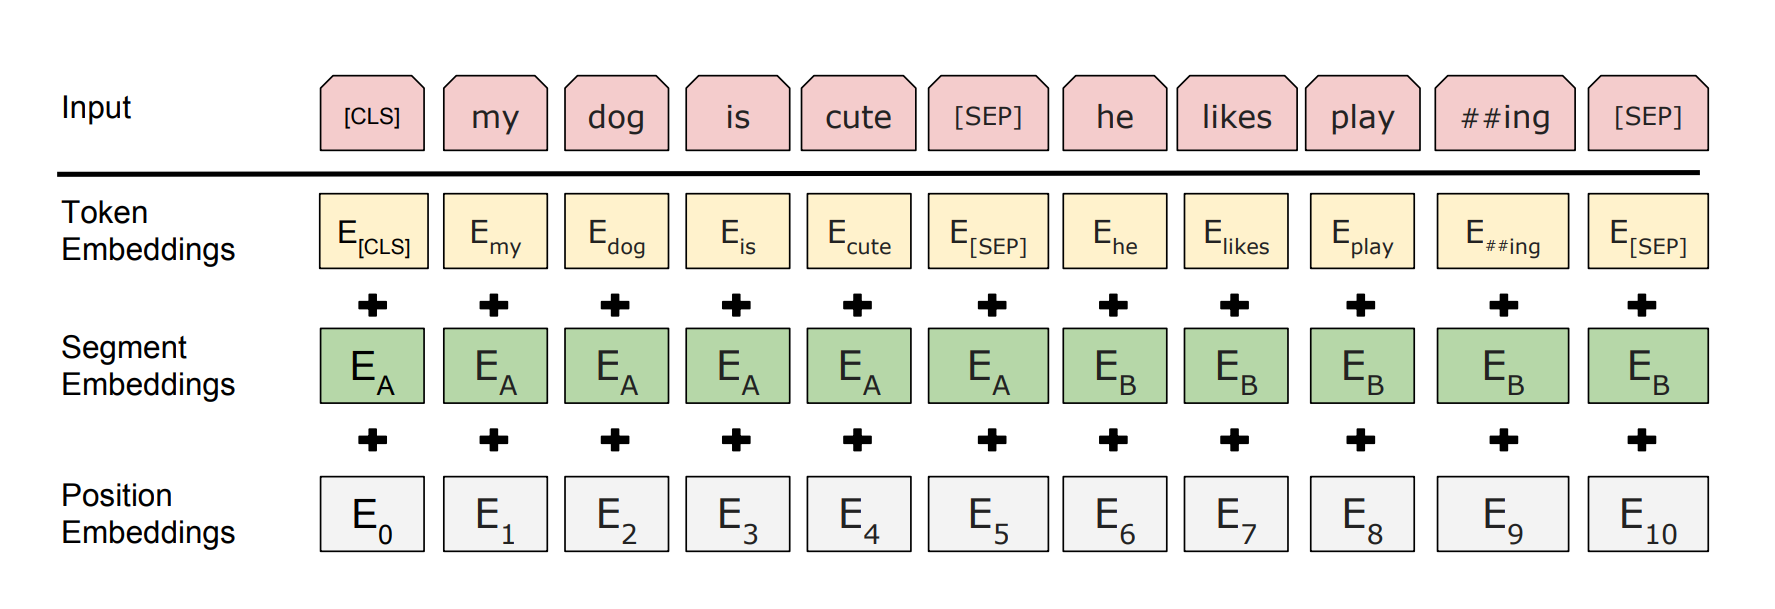
\includegraphics[width = 10cm]{figure/bert-input.png}\\ 
	\citebutton{Source: Devlin et al., 2019}{https://aclanthology.org/N19-1423.pdf}
\end{figure}

\begin{itemize}
	\item Two concatenated sentences as input
	\item WordPiece tokenization \citebutton{Wu et al., 2016}{https://arxiv.org/abs/1609.08144} for the inputs\\
			$\rightarrow$ Vocabulary of 30.000 tokens
	\item \textit{Learned} segment $+$ position embeddings
	\item Special \texttt{[CLS]} and \texttt{[SEP]} tokens
\end{itemize}

\vfill

\end{frame}

% ------------------------------------------------------------------------------

\begin{frame}{bert -- all embeddings}

\vfill

\begin{figure}
	\centering
	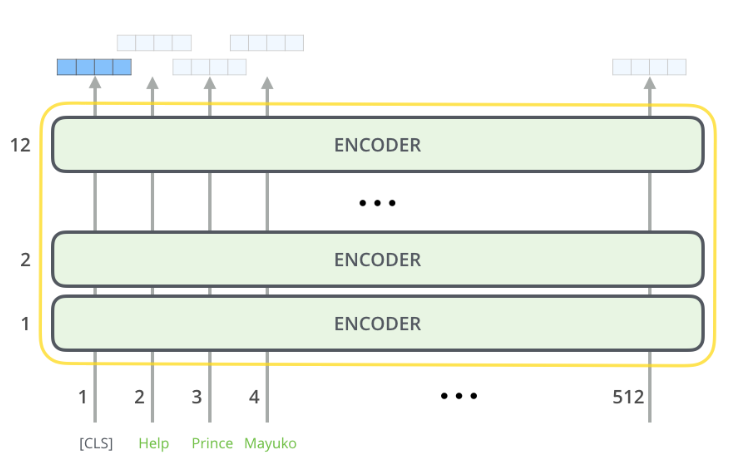
\includegraphics[width = 8cm]{figure/bert-embedings.png}\\ 
		\citebutton{Source: Jay Alammar}{https://jalammar.github.io/illustrated-bert/}
\end{figure}

\begin{itemize}
	\item One embedding per token per layer
	\item Non-contextual embeddings in the very first embedding layer
	\item More contextualization deeper into the model
\end{itemize}

\vfill

\end{frame}

% ------------------------------------------------------------------------------

\begin{frame}{bert -- the role of [CLS] and [SEP]}

\vfill

\textbf{Why deliberately include extra ``words``?}

\begin{itemize}
	\item The \texttt{[CLS]} token serves as an overall embedding for representing the whole sequence\\
				$\to$ Later on (cf. next chapter) BERT can thus used for classifying whole sequences\\
				$\to$ Can be extracted and used for clustering or similar
	\item The \texttt{[SEP]} (short for ```separator`) token serves as a ``signal`` for the model when used for taks on pairs of sequences
\end{itemize}

\textbf{Note:}

\begin{itemize}
	\item One further ``special`` token: \texttt{[UNK]} for representing unknown tokens or symbols (so the don't ``break`` the model)
\end{itemize}

\vfill

\end{frame}

% ------------------------------------------------------------------------------

\begin{frame}{Two different BERT versions}
\textit{There are two different BERT versions, namely BERT base and large. Depending on the architecture we get different parameter counts} \citebutton{Source: Devlin et al., 2019}{https://arxiv.org/abs/1810.04805}

\hspace{}

\begin{itemize}
	\item \textbf{BERT base:}
	\begin{itemize}
		\item $n_{layers} = 12$, we have 12 encoder layers
		\item $n_{heads} = 12$, this will not affect the parameter count since they perfectly split $d_{model}$ across the heads
		\item $d_{model} = 768$, thats the embedding dimension
	\end{itemize}

\hspace{}
	
	\item \textbf{BERT large:}
	\begin{itemize}
		\item $n_{layers} = 24$
		\item $n_{heads} = 16$
		\item $d_{model} = 1024$
	\end{itemize}
\end{itemize}
	
\end{frame}

%-------------------------------------------------------------------------------

\begin{frame}{Encoder Parameter Count}

\textit{From the chapter about the transformer parameter count we already know the number of parameters for one Encoder layer: $12\cdot d_{model}^2$}
$$
N_{Encoder} &= n_{layers} \cdot 12\cdot d_{model}^2
$$

\hspace{}

\begin{itemize}
	\item \textbf{BERT base}:
	$$N_{Encoder} = 12\cdot 12\cdot 768^2 = 84,934,656$$
	\item \textbf{BERT large}:
	$$N_{Encoder} = 24\cdot 12\cdot 1024^2 = 301,989,888$$
\end{itemize}

\hspace{}

\textit{By increasing $d_{model}$ and $n_{layers}$ we more than tripled the number of Encoder parameters!}
\end{frame}

%-------------------------------------------------------------------------------

\begin{frame}{Embedding Parameter Count}
\textit{Similar to the Transformer chapter we also have to consider the paramters from the embeddings:}

\hspace{}

\begin{itemize}
	\item Let $V$ be the vocabulary size, $M$ the maximum sequence length and $S$ the number of segments
	\item BERT has three kinds of embeddings, which are all learned:
	\begin{itemize}
		\item $V \times d_{model}$ token embeddings
		\item $S \times d_{model}$ segment embeddings
		\item $M \times d_{model}$ position embeddings
	\end{itemize}
	\item From the BERT paper we know $V=30000$, $S = 2$ and $M = 512$ 
	\item \textbf{BERT base}:
	$$N_{Embedding} = 30000\times 768 + 2\times 768 + 512\times 768 = 23,434,752$$
	\item \textbf{BERT large}:
	$$N_{Embedding} = 30000\times 1024 +2\times 1024 + 512\times 1024 = 31,246,336$$
\end{itemize}
	
\end{frame}

%-------------------------------------------------------------------------------

\begin{frame}{Final Parameter Count}
\textit{Now we just have to sum up both parts to get the final parameter count:}

\hspace{}

\begin{itemize}
	\item \textbf{BERT base}: 
	$$N_{Total} = 84,934,656 + 23,434,752 = 108,369,408 \approx 110M$$
	\item \textbf{BERT large}:
	$$N_{Total} = 301,989,888 + 31,246,336 = 333,236,224 \approx 340M$$
\end{itemize}
	
\end{frame}

% ------------------------------------------------------------------------------

\endlecture
\end{document}
